\label{capitolo5}
\section{Organizzazione fisica dei dati}
I DBMS hanno un architettura a livelli, tra cui il principale è il livello \emph{logico}, ovvero quello a cui fanno riferimento gli utenti, ed il livello \emph{fisico} che stabilisce, invece, realmente l'implementazione del DBMS.\\
Le relazioni vengono realizzate utilizzando varie strutture fisiche con molteplici varianti, ognuna delle quali favorisce alcune operazioni e ne penalizza altre.\\
La proprietà di \emph{indipendenza dei dati} permette agli utenti di ignorare la costruzione della struttura dati al punto che esse possono essere modificate senza variare i programmi che utilizzano questi dati.\\
Nelle applicazioni di basi di dati le operazioni sono specificate in SQL e vengono gestite da un particolare modulo chiamato \emph{gestore delle interrogazioni} che traduce le interrogazioni in una forma a più basso livello al fine di renderle più efficienti, per questo viene anche chiamato \emph{ottimizzatore delle interrogazioni}; a questo punto le interrogazioni in questa forma ottimizzata sono eseguite da un modulo sottostante chiamato \emph{gestore dei metodi d'accesso}. Questo modulo trasforma le interrogazioni in operazioni di lettura e scrittura che vengono eseguite dal \emph{gestore del buffer} che si occupa di mantenere e decidere quali pagine mantenere e caricare sulla memoria centrale. Nel caso il gestore del buffer abbia bisogno di pagine in memoria secondaria invia le richieste effettive di lettura e scrittura fisica al \emph{al gestore di memoria secondaria} vedi Fig. \ref{fig:schemod}
\begin{figure}
  \centering
  % Requires \usepackage{graphicx}
  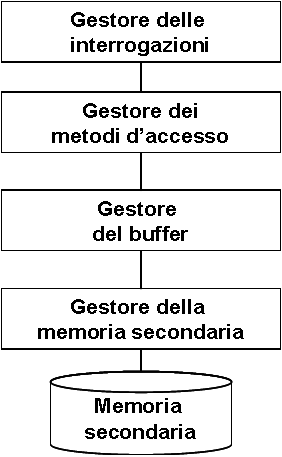
\includegraphics[width=5cm]{img/memsec.png}\\
  \caption{Schema dei moduli di gestione dei dati}\label{fig:schemod}
\end{figure}
\subsection{Memoria principale, memoria secondaria e gestione del buffer}
Le basi di dati hanno necessità di gestire dati in memoria secondaria per due motivazioni; la prima è che per quanto le dimensioni delle memorie centrali siano in costante aumento esse non riescono a soddisfare il fabbisogno della base di dati. In secondo luogo una delle caratteristiche delle basi di dati è la \emph{persistenza} e visto che le memorie centrali attualmente sono di tipo volatile non sono adatte a mantenere questa caratteristica.\\
Vediamo ora alcune caratteristiche della memoria secondaria, prima fra tutte come dice il nome stesso la memoria secondaria non può essere usata direttamente dai programmi, i dati per poter essere utilizzati devono prima essere caricati in memoria centrale. Sui dischi i dati sono memorizzati in \emph{blocchi} di dimensione (di solito) fissa di alcune decine di kilobyte. Le uniche operazioni possibili su un disco, come abbiamo già detto, sono le operazioni di lettura e scrittura di un intero blocco, questo significa che quando abbiamo bisogno anche di un solo bit dobbiamo caricare in memoria un intero blocco.\\
L'interazione tra memoria centrale e memoria secondaria è realizzata dai DBMS attraverso un apposita zona in memoria centrale detta \emph{buffer} gestita in modo condiviso dal DBMS per tutte le applicazioni. La gestione ottimale dei buffer è una questione essenziale in quanto permettono di evitare continui accessi alla memoria secondaria. Il buffer è organizzato in \emph{pagine} che hanno dimensione pari ad un numero intero di blocchi, per semplicità nel nostro caso imposteremo il numero di blocchi per pagina uguale a 1 e quindi non faremo distinzione tra i due termini.\\
Il \emph{gestore del buffer} si occupa del caricamento e dello scaricamento delle pagine dalla memoria centrale alla memoria di massa; possiamo pensare questo modulo come a un entità che riceve dai programmi richieste di lettura e scrittura su un blocco ed esegue le effettive letture e scritture sulla base di dati  secondo delle tempistiche che non coincidono con quelle di arrivo delle richieste; in particolare abbiamo che:
\begin{itemize}
  \item In caso di lettura, se la pagina è già presente nel buffer non è necessaria l'effettiva lettura fisica.
  \item In caso di scrittura il gestore può decidere di differire la scrittura fisica quando è possibile mantenere l'affidabilità del sistema.
\end{itemize}
Le politiche di gestione dei buffer assomigliano a quelle che il sistema operativo usa per la gestione della memoria centrale e obbediscono al principio di \emph{località dei dati} in base al quale i dati appena acceduti sono quelli con più alta probabilità che siano acceduti nell'immediato futuro.\\
La gestione del buffer è un po più complicata di così in quanto bisogna memorizzare informazioni sull'uso delle pagine che potremmo schematizzare nel seguente modo:
\begin{itemize}
  \item Un direttorio descrive il contenuto attuale del buffer indicano per ogni pagina quali sono il file fisico e il numero di blocchi ad essa corrispondenti.
  \item Per ogni pagina il gestore mantiene alcune variabili di stato fra cui un contatore dei programmi che usano quella pagina e un bit di stato per indicare se la pagina è stata modificata.
\end{itemize}
Un possibile insieme di operazioni che soddisfano queste caratteristiche sono le seguenti:
\begin{itemize}
  \item La primitiva \emph{fix} viene usata dalle transizioni per richiedere l'accesso ad una pagina e restituisce il riferimento alla pagina del buffer; l'esecuzione di tale operazione avviene nel seguente modo:
      \begin{enumerate}
        \item Si ricerca la pagina tra quelle già presenti in memoria, in caso positivo si ritorna l'indirizzo di memoria al richiedente
        \item Altrimenti si cerca una pagina libera del buffer cioè quelle con contatore pari a zero. Se il dirty bit è a uno allora essa viene scritta in memoria di massa.
        \item Se non esistono pagine libere possiamo avere due casi in base al comportamento del gestore del buffer, nel primo caso (politica \emph{steal}) viene sottratta una pagina ad un altra applicazione e la pagina viene scaricata in memoria di massa (operazione di \emph{flush}). Nel secondo caso (politica \emph{no steal}) la transizione viene sospesa fino alla liberazione di una pagina del buffer.
        \item In ogni caso quando viene effettuato un accesso alla pagina si incrementa il contatore relativo all'utilizzo di quella pagina.
      \end{enumerate}
  \item La primitiva \emph{setDirty} indica la modifica di una pagina e fa variare il bit relativo allo stato della pagina stessa
  \item La primitiva \emph{unfix} indica che il modulo chiamante ha terminato l'utilizzo della pagina e si ha come effetto il decremento del contatore.
  \item La primitiva \emph{force} forza il gestore del buffer a trascrivere in memoria la pagina in  modo sincrono
\end{itemize}
\subsection{Gestione delle tuple nelle pagine}
Sebbene ogni organizzazione fisica abbia una propria tecnica per la gestione delle pagine si sono alcuni aspetti comuni che possono essere interessanti da descrivere. In ciascuna pagina sono presenti due tipi di informazioni, l'informazione \emph{utile}, che coincide con i dati veri e propri e l'informazione di \emph{controllo} che consente di accedere alle informazioni.
\begin{figure}
  \centering
  % Requires \usepackage{graphicx}
  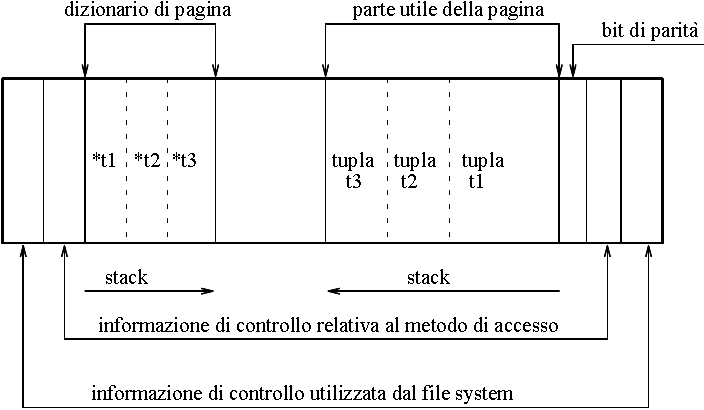
\includegraphics[width=15cm]{img/pagestr.png}\\
  \caption{Esempio di struttura di pagina}\label{fig:pagestr}
\end{figure}
Una possibile struttura di pagina è quella presentata in Fig. \ref{fig:pagestr} e qui descritta:
\begin{itemize}
  \item Ogni pagina, in quanto coincidente con un blocco ha una parte iniziale\emph{block header} e una finale \emph{block trailer} contente informazioni utilizzate dal filesystem.
  \item Ogni pagina in quanto contenete dati gestiti dal DBMS ha una parte iniziale (\emph{page header}) e una finale (\emph{page trailer}) contenenti informazioni di controllo specifiche alla struttura
  \item In molti casi ogni pagina ha un suo \emph{dizionario di pagina} che contiene un puntatore agli elementi della pagina e una \emph{parte utile} che contiene i dati. Dizionario di pagina e parte utile crescono solitamente come stack contrapposti lasciando così memoria libera in uno spazio contiguo.
  \item Infine ogni pagina contiene \emph{bit di parità} per verificare la correttezza dell'informazione.
\end{itemize}
In  molti casi non è possibile separare una tupla su più pagine così la massima dimensione della tupla è limitata a massimo spazio disponibile sulla pagine; in oltre molte volte le tuple hanno tutte quante la stessa dimensione, questo semplifica la struttura dei dizionari di pagina ma si corre il rischio di sprecare spazio nella pagina stessa.\\
Un parametro importante è il \emph{fattore di blocco} ovvero il numero di record contenuti in un blocco, che in prima approssimazione è pari al rapporto tra la dimensione del blocco e la dimensione media delle tuple.\\
Le primitive messe a disposizione dal gestore delle pagine sono:
\begin{description}
  \item[Inserimento e aggiornamento] che non comportano la riorganizzazione della pagina se esiste spazio sufficiente per la gestione della tupla. Se invece lo spazio non è contiguo le operazioni devono essere precedute da una riorganizzazione della pagina che però ha un costo limitato in quanto svolto in memoria centrale.
  \item[Cancellazione] essa è sempre possibile e viene fatta senza riorganizzare la pagina ma semplicemente marcando la tupla come "non valida".
  \item[Accesso a una tupla]  avviene tramite l'identificazione della valore della chiave o in base all'offset presente nel dizionario.
  \item[Accesso a un campo della tupla] identificato in base all'offset e alla lunghezza del campo stesso dopo aver identificato la tupla.
\end{description}
\subsection{Strutture primarie per l'organizzazione di file}
Le strutture con le quali vengono costruiti i file possono essere di tre tipi, \emph{sequenziali}, ad \emph{accesso calcolato} (o \emph{hash}) e ad \emph{albero}. Le strutture sequenziali sono caratterizzate da una struttura sostanzialmente consecutiva delle tuple in memoria di massa che deriva da una regola opportuna (istante di inserimento, valore di un campo).
Le strutture ad hash calcolano la posizione delle tuple in base ad un algoritmo. Le strutture ad albero, infine, sono utilizzate soprattutto come strutture secondarie.\\
\subsubsection{Strutture sequenziali}
Nelle strutture sequenziali un file è costituito da vari blocchi di memoria "logicamente" consecutivi e i le tuple vengono inserite nei blocchi rispettando una sequenza che può essere:
\begin{itemize}
  \item di tipo \emph{seriale (disordinata)} nel quale le tuple sono ordinate secondo l'ordine di immissione.
  \item un organizzazione ad \emph{array} nel quale le tuple sono disposte secondo il valore di un campo detto \emph{indice}.
  \item una organizzazione \emph{sequenziale ordinata} nel quale l'organizzazione dipende dal valore assunto in ciascuna tupla da un campo del file.
\end{itemize}
\paragraph{Struttura seriale (disordinata)}
In questo tipo di struttura gli inserimenti avvengono alla fine del file in modo sequenziale e sono perciò molto efficienti, basta gestire un puntatore all'ultima tupla inserita. I problemi si presentano nel caso di cancellazione e modifica di una tupla in quanto la cancellazione spreca memoria, mentre la modifica, nel caso di aumento di memoria, comporta una ristrutturazione dell'intero file.
Questa struttura è anche chiamata \emph{entry-sequence} per sottolineare il metodo di inserimento o \emph{heap} per specificare che i dati sono "ammucchiati" senza nessun ordine.\\
Questa tipo di struttura è molto efficiente per quanto riguarda letture e scritture ma molto meno efficiente quando si tratta della ricerca di un singolo dato all'interno del file. Per ovviare a questo problema, nelle basi di dati relazionali queste tipi di strutture (le più utilizzate visto la semplicità di implementazione e gestione) vengono affiancate da strutture secondarie.
\paragraph{Struttura sequenziale ad array} Le strutture ad array sono implementabili solo nel caso in cui le tuple siano di dimensioni fissa, in questo caso allora al file vengono associati \emph{n} blocchi contigui con $m$ spazzi per il salvataggio delle tuple dando luogo ad un array di dimensione $n\times m$ ciascuna tupla viene dotata di un indice $i$ e viene posta nella posizione $i$-esima dell'array.\\
Le primitive garantite da questa organizzazione sono quelle di inserimento, lettura e cancellazione; gli inserimenti iniziali avvengono semplicemente incrementando l'indice mentre le cancellazione lasciano delle posizioni libere, i successivi inserimenti vanno a riempire queste posizioni libere o avvengono in fondo al file.\\
Le strutture ad array non vengono quasi mai utilizzate nei DBMS in quanto, nella maggior parte dei casi, le tuple non rispettano le condizioni iniziali di questa struttura.
\paragraph{Struttura sequenziale ordinata} L'organizzazione sequenziale ordinata assegna a ciascuna tupla una posizione in base al valore di un campo detto \emph{chiave}. Sono così avvantaggiate le operazioni che richiedono un accesso ordinato alle tuple di una tabella in base alla chiave, ed inoltre è possibile effettuare ricerche dicotomiche.\\
Questo tipo di struttura non è più utilizzato in tempi recenti in quanto vi è un problema fondamentale nell'inserimento di nuove tuple che richiede un eccessivo overhead per la gestione di queste strutture. Infatti l'inserimento di una nuova tupla implica sempre o quasi sempre il riordino delle altre tuple. Alcuni meccanismi che possono migliorare questo problema sono:
\begin{itemize}
  \item Prevedere a priori un certo numero di posizioni libere all'atto del caricamento iniziale in modo da permettere un successivo riordino "locale".
  \item Inserire nuovi blocchi a seguito di saturazioni ma questa porta a rinunciare alla contiguità dei blocchi.
  \item integrare il file sequenziale ordinato con \emph{file di overflow} dedicato a gestire le tuple che eccedono lo spazio disponibile, i diversi file di overflow sono collegati tra loro da una \emph{catena di overflow} che parte da un blocco del file ordinato.
\end{itemize}
\subsubsection{Strutture ad accesso calcolato}
Una struttura ad accesso calcolato garantisce, come la struttura sequenziale ordinata, un accesso \emph{associativo} ai dati, ovvero il posizionamento fisico dei dati dipende da un valore assunto da un campo chiave; a differenza però della struttura sequenziale, quella ad hash, non necessita che i dati siano fisicamente sequenziali. La struttura viene realizzata allocando al file un numero $B$ di blocchi (sovradimensionando il file e non riempiendo completamente i blocchi si ottiene un funzionamento migliore).\\
L'idea è quella di estendere le caratteristiche di accesso degli array anche nel caso in cui questi non siano applicabili. Gli array si prestano a realizzare una struttura per organizzare dati che abbiano un campo chiave con valori consecutivi. Mentre nel caso nel caso il numero degli elementi è molto più piccolo dei valori possibili per il campo chiave la tecnica sequenziale degrada velocemente. Volendo però usare una struttura simili a quella degli array si può pensare di trasformare il campo chiave in un indice di un array; per fare ciò si utilizza un algoritmo e la funzione di trasformazione è detta \emph{funzione di hash}. Il problema principale di questo tipo di struttura è il fatto che il campo chiave è molto più grande dei possibili valori dell'indice e perciò la funzione di hash non può essere iniettiva ed è quindi possibile che si verifichino collisioni, ovvero chiavi con valori diversi ma che portano allo stesso valore di indice. Anche se una buona funzione di hash rende bassa la probabilità di collisione l'unico modo per abbassare effettivamente le collisioni è aumentare lo spazio disponibile.\\
Ora, traendo vantaggio dalla proprietà della memoria secondaria che l'operazione di accesso ad un blocco ha costo unitario e che un blocco può contenere diversi record, e dato che si tende a non riempire completamente un blocco ma si tende a mantenere un certo \emph{fattore di riempimento} per allocare la giusta quantità di blocchi per memorizzare un certo numero di record con una funzione di hash si può usare la formula:
$$B=\left\lceil\frac{T}{f \times F}\right\rceil$$
Dove $T$ è il numero di tuple previsto per il file $f$ è il fattore di riempimento e $F$ il fattore di blocco (numero di record per blocco).
In caso di collisione i record vengono semplicemente allocati nel blocco fino ad esaurimento dello spazio e quando questo è esaurito viene allocato un ulteriore blocco e i nuovi record vengono allocati in esso dando così luogo a \emph{catene di overflow}.\\
La struttura hash è ideale quando si vuole effettuare un \emph{accesso puntuale} ad un record tramite la sua chiave ma le prestazioni degradano pesantemente in caso di accesso ad un certo intervallo di valori della chiave in quanto la funzione di hash tende a disperdere i dati. Mentre non si ha alcun vantaggio quando si vuole accedere ad un qualsiasi altro campo della tupla.
\subsection{Strutture ad albero}
In questo paragrafo studieremo le strutture ad albero denominate \emph{indici}, esse sono strutture che favoriscono l'accesso in base al valore di uno o più campi sia nel caso di accessi puntuali sia nel caso di accessi ad intervalli. Le strutture ad albero possono essere utilizzate sia per la costruzione di strutture primarie, ovvero contenete i dati, sia strutture secondarie che favoriscono solamente gli accessi ai dati.\\
\subsubsection{Indici primari e secondari}
Daro un file $f$ con un campo chiave $k$ un \emph{indice secondario} è un altro file in cui ogni record è composto da due campi uno contenete un valore della chiave $k$ e l'altro contente l'indirizzo fisico del record in $f$. L'indice secondario è ordinato in base alla chiave perciò consente una rapida ricerca in base a quel valore. Nel caso in cui, invece, l'indice contiene al suo interno anche i dati esso è detto \emph{indice primario} perché non garantisce l'accesso solo in base alla chiave ma contiene anche i dati stessi. Un file può avere un solo indice primario e più indici secondari.\\
Della struttura ad albero possiamo analizzare alcune caratteristiche:
\begin{itemize}
  \item Nel primo caso gli indirizzi fisici si riferiscono solo ai blocchi di memoria nel quale il dato è contenuto, oppure possono contenere gli offset all'interno del blocco. Le due soluzioni se pur diverse sono paragonabili in termini di prestazioni. I puntatori ai blocchi sono più compatti mentre i puntatori ai record permettono di rendere più efficenti alcune interrogazioni.
  \item Un indice primario, grazie al suo ordinamento, può essere realizzato puntando ad un solo record per ciascun blocco; in questo caso si dice che l'indice è \emph{sparso}. In caso di indice secondario, invece, esso deve contenere per forza tutti i riferimenti della chiave visto che valori consecutivi della chiave possono trovarsi in blocchi differenti. in questo caso si parla di indice \emph{denso}.
\end{itemize}
Per quanto riguarda le prestazioni in ogni caso la caratteristica degli indici è quella di permettere ricerche efficienti sia nel caso di range che di singolo record, inoltre, gli indici sono solitamente più piccoli dei file a cui fanno riferimento e quindi le ricerche possono essere più efficienti.
\subsubsection{Strutture ad albero dinamiche}
Le strutture ad albero dinamiche del tipo \emph{B-tree} o \emph{B+-tree} sono le più usate nei DBMS relazionali per la realizzazione degli indici. Ogni albero ha un nodo radice, vari nodi intermedi e vari nodi foglia, ogni nodo coincide cono una pagina o blocco a livello di file system e di gestore del buffer. I legami tra i nodi vengono stabiliti da puntatori che collegano fra loro le pagine, ogni nodo ha un numero di discendenti abbastanza grande che dipende dall'ampiezza della pagina. Si costruiscono così alberi con un numero \emph{limitato di livelli} nei quali la maggioranza dei nodi è costituita da nodi foglia.\\
Un altro requisito fondamentale per un  buon funzionamento di queste strutture dati è che gli alberi siano \emph{bilanciati} ovvero che la lunghezza del cammino che collega il nodo radice con qualsiasi nodo foglia sia pressochè identica e pari alla profondità dell'albero.\\
\paragraph{Contenuto dei nodi e tecnica di ricerca}
\begin{figure}
  \centering
  % Requires \usepackage{graphicx}
  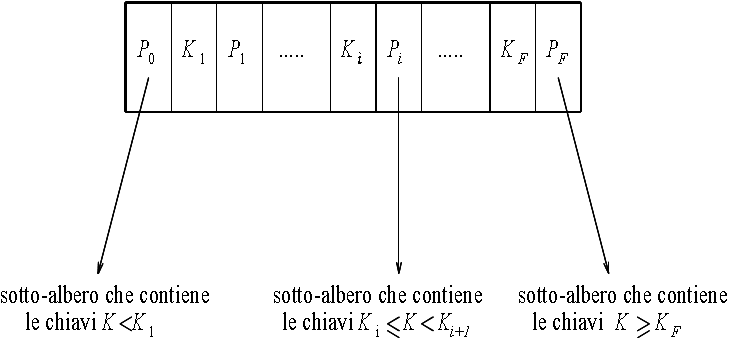
\includegraphics[width=14cm]{img/nodo.png}\\
  \caption{Esempio di nodo intermedio}\label{fig:nodo}
\end{figure}
La struttura tipica di un nodo è mostrata in figura \ref{fig:nodo}, esso presenta una sequenza di $F$ valori ordinati di chiave. Ogni chiave $K_i$ con $1\leq i \leq F$ è seguita da un puntatore $P_i$. $K_1$ è preceduta da un puntatore $P_0$. Ciascun puntatore punta ad un sotto-albero così definito:
\begin{itemize}
  \item Il puntatore $P_0$ punta al sotto-albero che contiene quei record con chiave \emph{minore} di $K_1$.
  \item Il puntatore $P_F$ indirizza al sotto-albero che contiene i record con chiavi \emph{maggiori o uguali} di $K_F$
  \item Gli altri puntatori puntano ciascuno ad un sotto-albero che contiene i  valori delle chiavi compresi tra i due valori $K_i$ e $K_{i+1}$
\end{itemize}
In sintesi ciascun nodo contiene $F$ valori di chiave e $F+1$ puntatori ad altri nodi, dove $F+1$ è detto \emph{fan-out} dell'albero; mentre $F$ dipende dall'ampiezza della pagina e dalla dimensione dei valori di chiave nella parte "utile" della pagina, si sceglie per $F$ il massimo valore possibile in modo da ridurre i livelli dell'albero.\\
La primitiva di ricerca nelle strutture ad albero è molto semplice in quanto consente un accesso associativo alla tupla che contiene la chiave $V$. Il meccanismo di ricerca consiste nel seguire i puntatori partendo dalla radice e considerando le seguenti regole:
\begin{itemize}
  \item se $V < K_1$ si segue il puntatore $P_0$
  \item se $V > K_F$ si segue il puntatore $P_F$
  \item altrimenti si segue il puntatore $P_j$ tale per cui $K_j \leq V <K_{j+1}$
\end{itemize}
e la ricerca prosegue fino ai nodi voglia dell'albero che possono essere organizzati nei due seguenti modi:
\begin{itemize}
  \item Nel primo caso i odi contengono l'intera tupla e la struttura dati che si ottiene è detta \emph{index-sequential} e permette la realizzazione di un file ordinato con un associato indice primario. La posizione della tupla è vincolata dal campo chiave. Cancellazione e inserimento non risultano però complicate in quanto la posizione viene stabilita dinamicamente.
  \item Nel secondo caso ciascun nodo foglia contiene puntatori ai blocchi della base di dati. La struttura che si ottiene in questo caso è detta \emph{indiretta}. La posizione delle tuple può essere qualsiasi e in questo caso si potrebbe indirizzarle con qualsiasi altro indice primario.
\end{itemize}
Inserimenti e cancellazioni non provocano grossi problemi nel caso in cui nel nodo vi sia spazio. Nel caso di inserimento in un nodo in cui non vi sia spazio a sufficienza si effettua un'operazione di \emph{split} che divide l'informazione già presente nella foglia più quella nuova in due foglie dal peso equilibrato. Questa operazione può provocare lo split anche ai nodi superiori fino a risalire la radice.\\
una cancellazione invece può essere sempre fatta in loco ma può portare a due problematiche:
\begin{itemize}
  \item Quando in un indice sparso la cancellazione coinvolge uno dei valori chiave è opportuno recuperare il successivo valore chiave e inserirlo al posto del valore cancellato.
  \item Quando una cancellazione lascia due foglie semivuote tanto che l'informazione in esse contenuta possa essere contenuta in una sola allora si deve svolgere un operazione di \emph{merge} che non è altro che il duale dell'operazione di split
\end{itemize}
\begin{figure}
  \centering
  % Requires \usepackage{graphicx}
  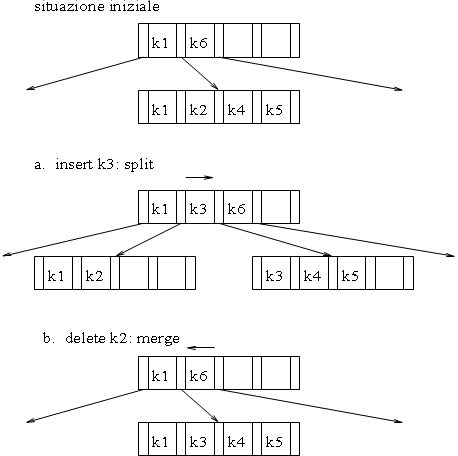
\includegraphics[width=10cm]{img/split.png}\\
  \caption{Esempio di operazioni di split (a) e di merge (b)}\label{fig:split}
\end{figure}
La modifica del valore di un campo chiave viene trattata come una cancellazione del suo valore iniziale seguito da un inserimento del valore finale.
\paragraph{Alberi B e B+}
Esistono due versioni della struttura ad albero, gli alberi di tipo B e quelli di tipo B+. La distinzione è abbastanza semplice, infatti, negli alberi di tipo B+ i nodi foglia sono collegati da una catena che li connette in base all'ordine della chiave; questo fa si che le interrogazioni il cui predicato definisce un intervallo di valori siano svolte in modo efficiente. In questo caso è sufficiente trovare il primo valore dell'intervallo per poi scandire il resto dei risultati in sequenza (Fig. \ref{fig:B+tree}).\\
Nel caso degli alberi di tipo B è possibile effettuare una ottimizzazione aggiungendo ad ogni chiave un puntatore che punta direttamente al record mentre l'altro puntatore punta al sottoalbero per continuare la ricerca (Fig. \ref{fig:Btree})
\begin{figure}
  \centering
  % Requires \usepackage{graphicx}
  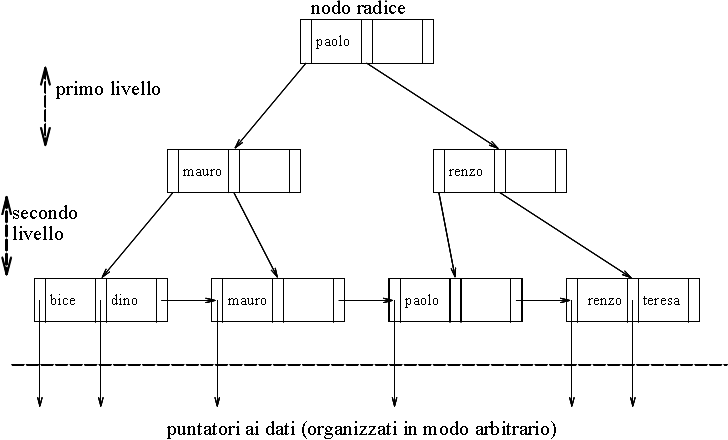
\includegraphics[width=12cm]{img/bptree.png}\\
  \caption{Albero di tipo B+}\label{fig:B+tree}
\end{figure}
\begin{figure}
  \centering
  % Requires \usepackage{graphicx}
  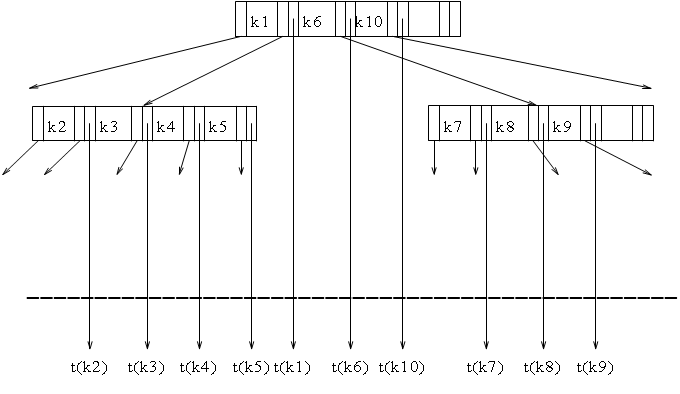
\includegraphics[width=12cm]{img/btree.png}\\
  \caption{Albero di tipo B}\label{fig:Btree}
\end{figure}
\subsection{Strutture fisiche e indici nei DBMS relazionali}
I DBMS attualmente in commercio differiscono in modo sostanziale per i dettagli sulle strutture fisiche che mettono a disposizioni, ma possiamo trovare alcuni principi generali sui quali la maggior parte dei DBMS si basa.\\
in particolare, tutti i sistemi prevedono una struttura di base di tipo seriale disordinata su cui è possibile definire inidici secondari. Quasi tutti i sistemi creano un indice per la chiave primaria in quanto questo rende più semplice verificare il rispetto del vincolo.
Molti sistemi prevedono la possibilità di memorizzare in modo contiguo le tuple di una tabella con gli stessi valori su un certo campo, questa tecnica prende il nome di \emph{cluster}. In molti casi si tratta di un vero e proprio ordinamento fisico, in altri è associata ad una funzione di hash o ad un indice.\\
Tutti i sistemi permettono la realizzazione di indici e praticamente tutti prevedono la realizzazione tramite B+-tree, mentre alcuni sistemi prevedono anche altri tipi di indice. Un altro tipo di indice è il cossiddetto \emph{indice hash} ovvero una struttura secondaria realizzata tramite l'accesso calcolato.
\subsection{Gestore delle interrogazioni: esecuzione e ottimizzazione}
Il gestore delle interrogazioni è un modulo cruciale dell'architettura di un DBMS in quanto responsabile dell'esecuzione \emph{efficiente} dell'operazioni che sono specificate a livello molto alto. Esso riceevve in ingresso un interrogazione SQL essa viene analizzata per indivuduare eventuali errori sintattici o semantici; in questa fase il sistema accede al \emph{dizionario dei dati} per leggere le informazioni in esso contenute ed effettuare i controlli. Una volta accettata l'interrogazione viene tradotta in una forma interna di tipo algebrico. A questo punto inizia la fase di ottimizzazione:
\begin{itemize}
  \item Viene svolta in primo luogo un'ottimizzazione di tipo algebrico che consiste nell'effettuare tutte le trasformazioni algebriche necessarie. Questa ottimizzazione avviene indipendentemente dal modello dei costi assunto dal sistema.
  \item In secondo luogo, viene svolta una ottimizzazione che dipende sia dalla tipologia dei metodi di accesso ai dati sia dal modello dei costi.
  \item Infine si genera il codice che utilizza i metodi di accesso ai datti, ovvero, si ottengono i \emph{programmi di accesso} in formato "interno" che richiedono l'uso delle strutture dati fornite dal sistema.
\end{itemize}
Al contrario di altri moduli l'ottimizzazione delle interrogazioni agisce a tempo di compilazione. Nel caso in cui l'interrogazione venga compilata una sola volta ed eseguita molteplici (\emph{complie and store}) il codice viene memorizzato nella base di dati. Nel caso in cui l'interrogazione venga compilata e immediatamente eseguita (\emph{compile and go}) il codice non viene memorizzato.
\subsubsection{Profili delle relazioni}
Ciascun DBMS contiene informazioni quantitative relative alle caratteristiche delle tabelle dette \emph{profili delle relazioni} che vengono memorizzate nel dizionario dei dati, alcuni di questi profili sono:
\begin{itemize}
  \item La \emph{cardinalità}, $CARD(T)$, ovvero il numero di tuple di ciascuna tabella T.
  \item La \emph{dimensione} in byte, $SIZE(T)$, di ciascuna tupla di T.
  \item La \emph{dimensione} in byte, $SIZE (A_j,T)$ di ciascun attributo di T.
  \item Il \emph{numero di valori distinti}, $VAL(A_j,T)$ di ciascun attributo $A_j$ di T.
  \item Il \emph{valore minimo}, $MIN(A_j,T)$, e quello \emph{massimo}, $MAX(A_j,T)$ di ciascun attributo di T.
\end{itemize}
I profili vengono calcolati in base ai dati effettivamente memorizzati nella tabella tramite l'ausilio di opportune primitive di sistema, ma è compito dell'amministratore richiamare periodicamente \texttt{update statics} per aggiornare questi profili.
\subsubsection{Rappresentazione interna delle query}
La rappresentazione che viene data dall'pttimizzatore ad una interrogazione tiene conto della struttura fisica utilizzata per implementare le tabelle, nonché degli indici disponibili su di esse. Perciò la prima trasformazione consiste nel rappresentare l'interrogazione con una struttura ad albero nella quale i nodi foglia corrispondono a strutture fisiche (tabelle, indici, file) e i nodi intermedi sono aoperazioni di accesso ai dati che sono supportati dalle strutture fisiche.
\paragraph{Operazione di scansione}
Un'operazione di \emph{scansione} (\emph{scan}) esegue diverse operazioni sia di ti tipo algebrico che non algebrico:
\begin{itemize}
  \item proiezione su di una lista di attributi
  \item selezione di un predicato
  \item inserimento cancellazioni e modifiche delle tuple quando vi si fa accesso durante la scansione
\end{itemize}
Le primitive che interessano questa operazione sono:
\begin{center}
  \texttt{open, next, read, modify, insert, delete,close}
\end{center}
\paragraph{Ordinamenti}
La necessità di operazioni di ordinamento emerge sia ai fini delle applicazioni (eseguite per lo più in memoria centrale tramite meccanismi ad hoc) sia per una corretta realizzazione di proiezioni con eliminazione dei duplicati (spesso eeseguita su grandi file tramite la composizione di sort su parti dei file e merge finale).
\paragraph{Accesso diretto}
 Si usa il termine \emph{accesso diretto} quando è possibile accedere ad uno o più record senza dover necessariamente esaminare il file in modo sequenziale, ma tramite indici; questo si ha nel caso in cui i predicati siano semplici ($A_i = V$) o intervalli ($V_1<A_i<V_2$), in questi casi si dice che il predicato dell'interrogazione è \emph{valutabile} tramite l'indice.\\
 Nel caso l'interrogazioni presenti un solo predicato valutabile la convenienza è quella di effettuare la ricerca tramite indice. Nel caso sia una \emph{congiunzione} di predicati valutabili allora si sceglie il più selettivo per l'accesso diretto mentre il secondo viene valutato in memoria centrale tramite \emph{scan}. Nel caso in cui l'interrogazione presenti una \emph{disgunzione} dei predicati basta che uno solo non sia valutabile che si rende necessaria una ricerca tramite scan.
 \paragraph{Metodo di join}
\begin{figure}
  \centering
  % Requires \usepackage{graphicx}
  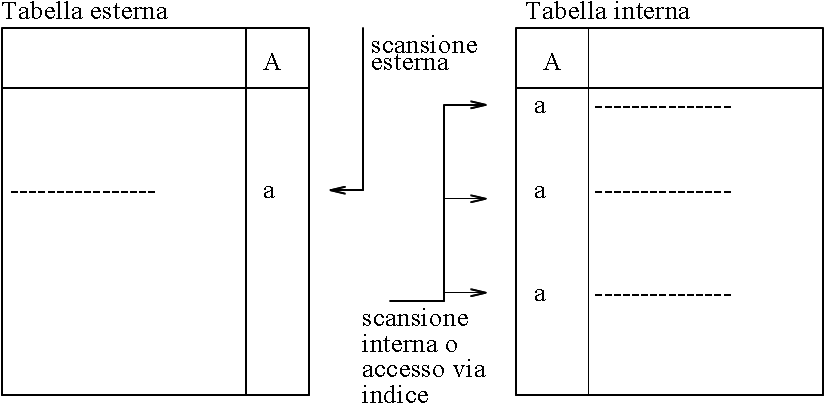
\includegraphics[width=13cm]{img/nested.png}\\
  \caption{Nested-loop join}\label{fig:nested}
\end{figure}
\begin{figure}
  \centering
  % Requires \usepackage{graphicx}
  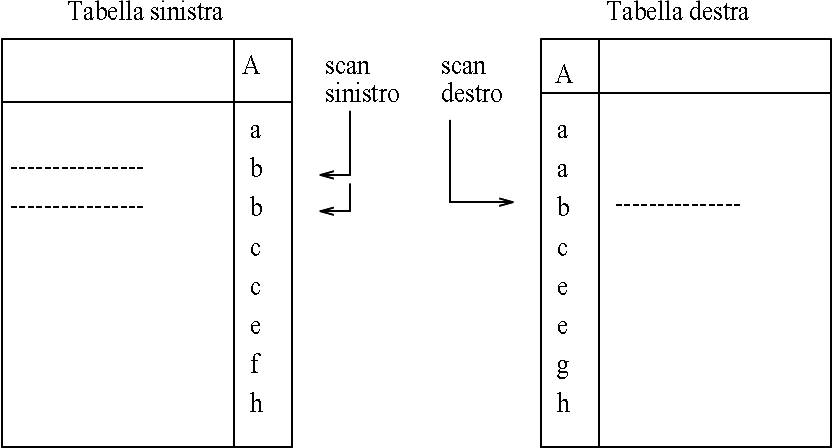
\includegraphics[width=13cm]{img/merge.png}\\
  \caption{Merge-scan join}\label{fig:merge}
\end{figure}
\begin{figure}
  \centering
  % Requires \usepackage{graphicx}
  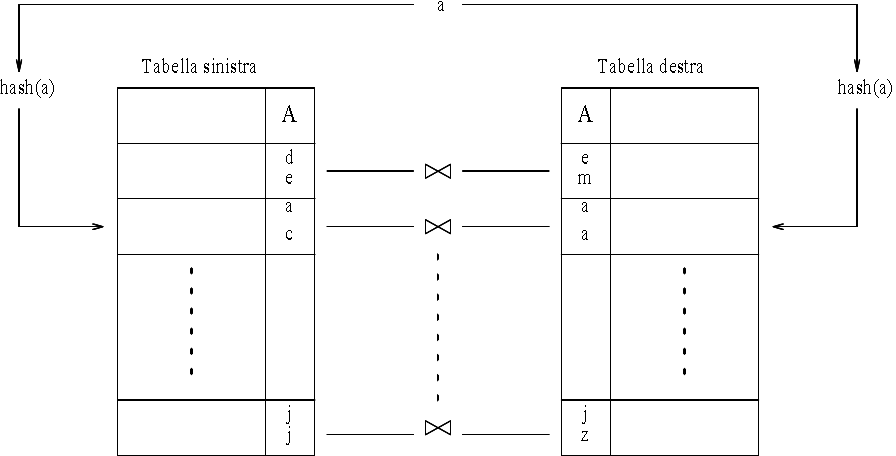
\includegraphics[width=13cm]{img/hashed.png}\\
  \caption{Hashed join}\label{fig:hashed}
\end{figure}
 Il join è l'operazione più costosa per un DBMS in quanto vi è il rischio di una esplosione del numero di tuple del risultato; un join su campi che non siano chiave per nessuno dei due operandi può avere un numero di tuple uguale al prodotto della cardinalità degli operandi stessi.\\
 Vediamo ora tre tipologie di realizzazione del join
 \begin{description}
   \item[Nested loop] Nel nested loop (Fig. \ref{fig:nested}) una tabella viene definita come \emph{esterna} mentre l'altra come \emph{interna}. Si esegue una scansione sulla tabella esterna e per ogni tupla individuata si preleva il valore dell'attributo e si ricerca tale valore nella tabella interna tramite una scansione o l'utilizzo di un indice \emph{ad hoc} sull'attributo cercato. Questa tecnica non ha un costo fisso ma dipende dalla disponibilità di spazio nel buffer e della tecnica di ricerca nella tabella interna
   \item[Merge scan] Questa tecnica (Fig. \ref{fig:merge}) richiede di esaminare le tabelle secondo l'ordine dell'attributo di join ed è quidi efficente quando le tabelle sono già ordinate o esistono degli indici adeguati. Viene eseguita mediante scansioni parallele sulle due tabelle come nei classici algoritmi di \emph{merge}; quando gli attributi coincidono allora vengono generate ordinatamente tuple del risultato
   \item[Hash-based] Questo metodo rapprfesentato in Fig. \ref{fig:hashed} viene eseguito in due passi: nel primo passo una funzione di hash $h$ applicata sugli attributi di join viene utilizzata per creare una copia ordinata di ciascuna delle due tabelle. La funzione $h$ fa corrispondere i valori di dominio di tali attributi a $B$ partizioni su ciascuna tabella. Le tuple con gli stessi valori dell'attributo di join saranno poste nelle stesse partizioni. Sarà così poi sufficiente effettuare B semplici join tra le partizioni a pari indice.
 \end{description}
 Il costo di queste tecniche non può essere valutato in astratto a priori ma dipende dalle scelte che precedono o seguono il join.
 \subsubsection{Ottimizzazione basata sui costi}
 L'ultimo passaggio che porta a definire il piano di accesso è assai difficile sul piano computazzionale in quanto sono presenti varie dimensioni di ottimizzazione.
 \begin{itemize}
   \item Occorre scegliere quali operazioni di accesso ai dati svolgere, in particolare, nel primo accesso ai dati occorre talvolta scegliere tra una scansione e un accesso tramite indici. 
   \item Occorre scegliere l'ordine delle operazioni da compiere
   \item Quando è possibile occorre scegliere fra le varie alternative per la realizzazione di una operazione (esempio il metodo di join)
   \item Quando l'interrogazione o il metodo di realizzazione richiedono un ordinamento bisogna stabilire a quale livello della strategia svolgere tale operazione.
 \end{itemize}
 Di fronte a questa complessità gli ottimizzatori dispongono di formule di costo approssimate. Essi costrruiscono un \emph{albero delle alternative} (Fig. \ref{fig:alterna}) in cui ogni nodo corrisponde a fissare una particolare opzione fra quelle elencare sopra. Ogni nodo foglia dell'albero corrisponde ad una specifica \emph{alternativa di esecuzione} della interrogazione descritta dalle scelte che si trovano percorrendo l'albero dalla radice fino al nodo foglia. Il problema è così riformulato nella ricerca del nodo foglia con costo minore.\\
\begin{figure}
  \centering
  % Requires \usepackage{graphicx}
  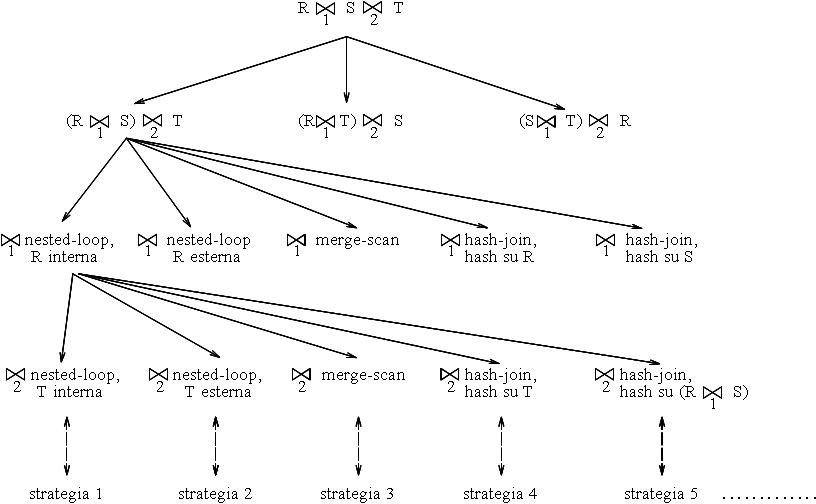
\includegraphics[width=12cm]{img/alterna.png}\\
  \caption{Albero delle alternative per un join su tre tabelle}\label{fig:alterna}
\end{figure}
 Il problema viene tipicamente risolto tramite formule di costo che associano a ciascuna operazione intermedia un costo in termini di operazioni di I/O e di istruzioni necessarie a valutarne il risultato.
 $$C_{total} = C_{I/O} \times n_{I/O} + C_{cpu} \times n_{cpu}$$
 Dove $C_{I/O},\ C_{cpu}$ sono parametri noti e $n_{I/O},\ n_{cpu}$ indicano il numero di operazioni di ingresso uscita e di istruzioni necessarie per valutare il risultato dell'interrogazione.\\
 Talvolta la strategia ottimale richiede la realizzazione di strutture ad hoc per svolgere le operazioni, in questo caso sono da considerare anche i costi di costruzione di tali strutture. 